
\mysection{Introduction}

Vu par l’extérieur, un manipulateur polyvalent pourrait sembler une technologie
plutôt inoffensive, pas très différent d’un tapis roulant ou d’une perceuse, mais
l’aspect innovative de ce type de machine est précisément sa polyvalence. Étant
reprogrammable, le manipulateur n’est pas limité à une utilisation particulière, ce
qui veut dire que le fabricant n’a pas besoin de traiter des considérations
particulières d’une industrie donnée, mais seulement avec des aspects généraux
(vitesse maximale, couple maximale, déplacement maximum, etc).
Le but de ce travail est précisément d’explorer cet aspect polyvalent d’un
manipulateur en proposant un système qui permet l’utilisateur de commander la
position de l’extrémité du manipulateur e ses trajectoires, ensuite on proposera une
application simple pour ce système, dont le but est de démontrer son
fonctionnement et évaluer sa performance. Le système complet est schématisé de
forme simplifiée ci-dessous: 

\begin{figure}[H]
	\begin{center}	
		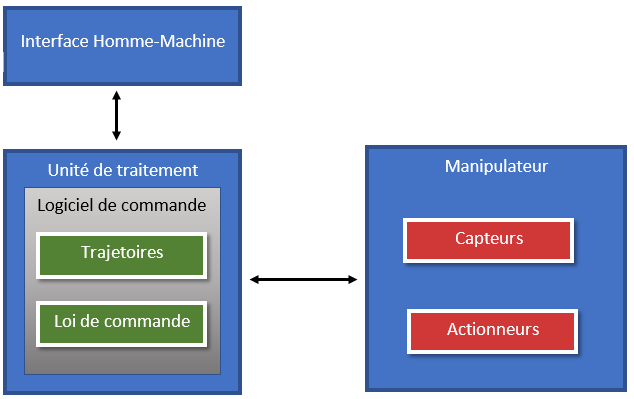
\includegraphics[width=10cm]{./IntroImage}
		\caption{Schéma simplifié du système.}
		\label{fig:Schema}
	\end{center}
\end{figure}